\chapter{The Virtual Observatory}

The International Virtual Observatory Alliance (IVOA) was formed in 2002 with the aim to "facilitate the international coordination and collaboration necessary for the development and deployment of the tools, systems and organizational structures necessary to enable the international utilization of astronomical archives as an integrated and interoperating virtual observatory." \footnote{\url{http://www.ivoa.net/}} The IVOA now comprises programs from Argentina, Armenia, Australia, Brazil, Canada, China,  France, Germany, Hungary, India, Italy, Japan, Russia, Spain, the United Kingdom, Ukraine, and the United States and inter-governmental organizations (ESA and ESO). Membership is open to other national and international programs according to the IVOA Guidelines for Participation.\\

The IVOA focuses on the development of standards and encourages their implementation for the benefit of the worldwide astronomical community. Working Groups are constituted with cross-program membership in those areas where key interoperability standards and technologies have to be defined and agreed upon. The Working Groups develop standards using a process modeled after the World Wide Web Consortium, in which Working Drafts progress to Proposed Recommendations and finally to Recommendations. Recommendations may ultimately be endorsed by the Virtual Observatory Working Group of Commission 5 (Astronomical Data) of the International Astronomical Union. The IVOA also has Interest Groups that discuss experiences using VO technologies and provide feedback to the Working Groups. Ad-hoc and permanent committees deal with specific scientific and procedural topics. Interaction with other scientific disciplines interested in data inter-operability is also pursued through dedicated Liaison Groups.\\

A chair is chosen from among the representatives and serves an eighteen-month term, normally preceded by an eighteen-month term as deputy chair. The Executive Committee meets 3-4 times a year and its members represent their respective programs and are expected to be in a position to commit resources targeted at the achievement of common goals. Decisions by the IVOA Executive Committee are reached by consensus. The IVOA holds two Interoperability Workshops each year. These meetings are opportunities for the IVOA Groups and Committees to have face-to-face discussions.\\

In this section we are not going to make a deep study of the Virtual Observatory techniques, technologies, protocols and interfaces, just those needed and selected to explain our proposal of including NoSQL into VO. Bearing in mind that the problem we are trying to address is data modelling, we will just make an overview of those aspects related with our work.\\

\section{ObsTAP}

A data model is a description of the objects represented by a computer system with their properties and relationships, a logical model detailing the decomposition of a complex dataset into simpler elements, like a collection of concepts and rules used in defining data model.\\

In 2011 IVOA proposed a new recommendation: Observation Data Model Core Components and its Implementation in the Table Access Protocol \footnote{\url{http://www.ivoa.net/documents/ObsCore/20110502/PR-ObsCore-v1.0-20110502.pdf}}. That document was intended to be a description of the interface which integrated the data modeling and data access aspects in a single service:\\ 

\doublebox{ObsCore data model + Table Access Protocol = ObsTAP}

\subsection{ObsCore Data Model}

This is the first block for ObsTAP.

\subsection{Table Access Protocol}

This is second block for ObsTAP, and defines a Web service for accessing tables containing astronomical catalogues. TAP is the protocol which underlies in the process of posing a query against a data source (or several data sources). The result of a query is a table, usually a VOTable. \footnote{Support for VOTable output is mandatory, while other formats may be available.}\\ 

Queries which use TAP protocol can be made through several clients, like:
\begin{itemize}
\item TOPCAT
\item TAPHandle which operates fully within the Web browser
\item The TAP shell, a command line interface to querying TAP servers, complete with metadata management and command line completion.
\item The GAVO VOTable library, which allows embedding TAP queries in Python.
\end{itemize}

The types of queries implemented by TAP are:

\begin{itemize}
\item Data queries
\item Metadata queries
\item Virtual Observatory Support Interface (VOSI)
\end{itemize}


TAP includes support for multiple query languages, including queries specified using the Astronomical Data Query Language (ADQL [1]) and the Parameterised Query Language (PQL, under development). Other query languages are also supported, and this mechanism allows developments outside the IVOA to be used without modifying the TAP specification.\\

Finally, it also includes support for both synchronous and asynchronous queries. Special support is provided for spatially indexed queries using the spatial extensions in ADQL.\\


\begin{lstlisting}
SELECT centerAlpha, centerDelta, dateObs FROM lsw.plates
  WHERE dateObs BETWEEN '1903-01-12' AND '1903-01-19'; 
\end{lstlisting}
ADQL Query for locating an unexpected object on the night sky between January 12th and 18th, 1903.


\section{Flexible Image Transport System}
 
Flexible Image Transport System (FITS) is an open standard defining a digital file format useful for storage, transmission and processing of scientific and other images. FITS is the most commonly used digital file format in astronomy. Unlike many image formats, FITS is designed specifically for scientific data and hence includes many provisions for describing photometric and spatial calibration information, together with image origin metadata.\\

The FITS format was first standardized in 1981; it has evolved gradually since then, and the most recent version (3.0) was standardized in 2008. FITS was designed with an eye towards long-term archival storage, and the maxim once FITS, always FITS represents the requirement that developments to the format must be backwards compatible.\\
 
A major feature of the FITS format is that image metadata is stored in a human-readable ASCII header, so that an interested user can examine the headers to investigate a file of unknown provenance. The information in the header is designed to calculate the byte offset of some information in the subsequent data unit to support direct access to the data cells. Each FITS file consists of one or more headers containing ASCII card images (80 character fixed-length strings) that carry keyword/value pairs, interleaved between data blocks. The keyword/value pairs provide information such as size, origin, coordinates, binary data format, free-form comments, history of the data, and anything else the creator desires: while many keywords are reserved for FITS use, the standard allows arbitrary use of the rest of the name-space.\\
 
FITS is also often used to store non-image data, such as spectra, photon lists, data cubes, or even structured data such as multi-table databases. A FITS file may contain several extensions, and each of these may contain a data object. For example, it is possible to store x-ray and infrared exposures in the same file.\\
 
FITS support is available in a variety of programming languages that are used for scientific work, including C, C++, C\#, Fortran, IGOR Pro, IDL, Java, LabVIEW, Mathematica, MatLab, Perl, PDL, Python, R, and Tcl. The FITS Support Office at NASA/GSFC maintains a list of libraries and platforms that currently support FITS.\\
 
Image processing programs such as ImageJ, GIMP, Photoshop, XnView and IrfanView can generally read simple FITS images, but frequently cannot interpret more complex tables and databases. Scientific teams frequently write their own code to interact with their FITS data, using the tools available in their language of choice. The FITS Liberator software is used by imaging scientists at the European Space Agency, the European Southern Observatory and NASA. The SAOImage DS9 Astronomical Data Visualization Application is available for many OSs, and handles images and headers.

\subsubsection{FITS Data Format}

A FITS file is comprised of parts called Header Data Units (HDU), being the first HDU called primary HDU o primeray array. This array can contain a 1-999 dimensional array. A typical primeray array could contain a 1D spectrum, 2D image or 3D data cube. Any number of HDU can follow the main array, and are called FITS extensions. Currently, three different¡ extensions can be defined:

\begin{itemize}
\item Image extension, a 0-9999 dimensional array of pixels, which begins with XTENSION = 'IMAGE'
\item ASCII table extension which stores tabular data in ASCII formats. They begin with XTENSION = 'TABLE'
\item Binary table extension stores tabular data in binary representation. Headers start with XTENSION = 'BINTABLE'
\end{itemize}

Besides, there are additional type of HDU called random groups, but only used for radio interferometry.
      
\begin{figure}[H]
\centering
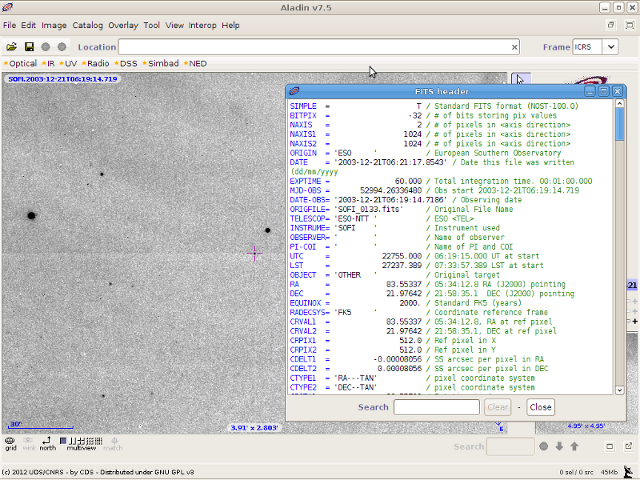
\includegraphics[width=11cm,height=8cm]{images/fits_header.png}\\
\caption{Viewing FITS header in Aladin}
\end{figure}






%%% Los cap'itulos inician con \chapter{T'itulo}, estos aparecen numerados y
%% se incluyen en el 'indice general.
%%
%% Recuerda que aqu'i ya puedes escribir acentos como: 'a, 'e, 'i, etc.
%% La letra n con tilde es: 'n.

%\chapter{OpenCADC}
\section{OpenCADC}
Esto es una prueba

\section{OpenCADC}

\textit{This research used the facilities of the Canadian Astronomy Data Centre operated 
by the National Research Council of Canada with the support of the Canadian Space Agency}.\\

OpenCADC (Canadian Astronomy Data Center) is a Virtual Observatory, used in ALMA Science Archive (for this reason is included in this chapter) tool which comprises several projects \footnote{We do not enumerate all of them here, for a full list, go to \url{https://code.google.com/p/opencadc/source/browse}}:

\subsection{Universal Worker Service}

The Universal Worker Service (UWS) pattern defines how to build asynchronous (the client does not wait for each request to be fulfilled; if the client disconnects from the service then the activity is not aborted), stateful (the service remembers results of a previous activity), job-oriented (the rules for setting and arranging the parameters for a job is called Job Description Language- JDL) services.

\begin{figure}[H]
\centering
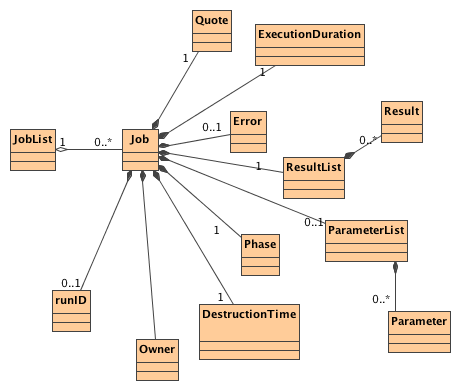
\includegraphics[width=11cm,height=8cm]{images/Class_Diagram__UWS__UWSObjects.png}\\
\caption{UWS Objects in class diagram}
\end{figure}

When the execution starts, the job is seen as a state machine which can adopt several states. The phases are the following:

\begin{itemize}

\item 
    PENDING: the job is accepted but not committed for execution by the client.
\item
    QUEUED: the job is committed for execution by the client but the service has not yet assigned it to a processor.
\item
    EXECUTING: the job has been assigned to a processor and the results can be produced at any time during this phase.
\item
    COMPLETED: execution is over and the user can collect the results.
\item
    ERROR: the job failed to complete.
\item
    ABORTED: the job has been stopped by the user or by the system.
\item
    UNKNOWN: the job is in an unknown state.
\item
    HELD: the job is pending execution.
\item
    SUSPENDED: The job has been suspended by the system during execution. This might be because of temporary lack of resource. Similar to aborted but in this state the UWS will automatically resume the when resource are available again.

\end{itemize}



\begin{figure}[H]
\centering
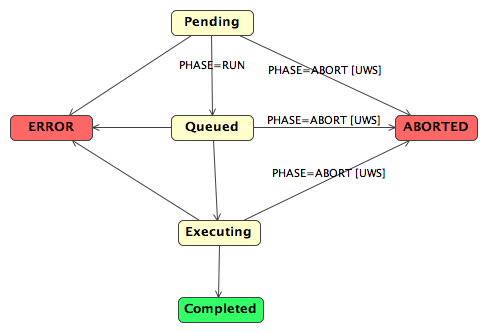
\includegraphics[width=11cm,height=8cm]{images/UWSStates.png}\\
\caption{Universal Worker Server Job states}
\end{figure}

Now, we make a subtle description of the structure of the code relating UWS in OpenCADC (the cadcUWS Library), the section of the code provides Job class and plugin architecture, servlet with UWS async and sync behaviour.

\subsubsection{JobManager}

Responsible for job control.

\subsubsection{JobPersistence}

In charge of storing and retrieving Job state.

\subsubsection{JobExecutor}

It executes every job in separated threads.

\subsubsection{JobRunner}

The code that actually executes the job.


\subsection{cadcTAP Library}

The cadcTAP library is responsible of async and sync queries, where QueryRunner implements JobRunner. It also contains TAP\_SCHEMA DDL statements and is used by query parser to validate table and column usage.

\subsubsection{TapQuery Interface}

It has a separate implementation for each LANG (e.g. $LANG = ADQL$) specified and processess the query to local SQL.

\subsubsection{SqlQuery}

When code states $LANG=SQL$, it implements TapQuery and fully navigates it ($FROM, WHERE$ and $HAVING$ clauses).

\subsubsection{AdqlQuery}

Same as before when $LANG=ADQL$.

\subsubsection{Plugins}

\begin{itemize}
\item UploadManager
\item TableWriter
\item FileStore
\end{itemize}


\subsubsection{QueryRunner}

It implements JobRunner and sets Job state, find DataSource and uses TapSchema, UploadManager, TapQuery and TableWriter.

